\vspace{-2.5\baselineskip}
\section{Plattformen}
\vspace{-0.8\baselineskip}
\begin{minipage}{0.4\textwidth}
\flushleft{}
    \vspace{-0.8\baselineskip}
    \subsection{Auswahl der Zielplattform}
    \begin{itemize}
        \item was muss gerechnet werden?
        \vspace{-0.8\baselineskip}
        \item wie schnell?
        \vspace{-0.8\baselineskip}
        \item wie viel Adressraum?
    \end{itemize}
    Erst wenn das feststeht $\rightarrow$ Peripherie miteinbeziehen (Grund: zu jeder CPU gibt es meist unzählige Varianten der Peripherie!)
\end{minipage}
\begin{minipage}{0.6\textwidth}
    \subsection{Vergleich der Beispielarchitekturen}
    \vspace{-1.5\baselineskip}
    \begin{multicols}{2}
        MSP430: Blockschaltbild\\
	    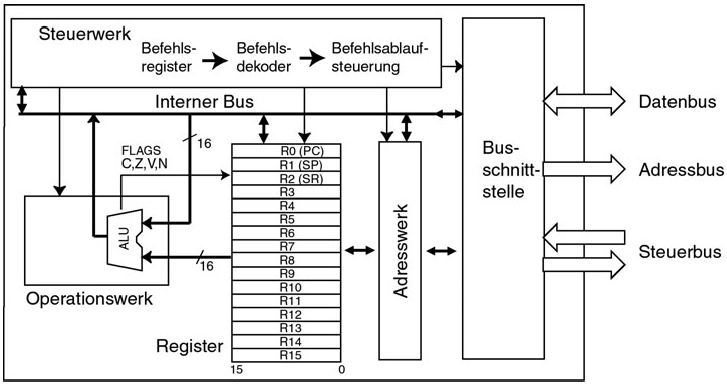
\includegraphics[width = 1.2\linewidth]{images/Plattformen/MSP430Blockschaltbild}
	\columnbreak
    	\flushright{}
	    CPU08: Registersatz\\
	    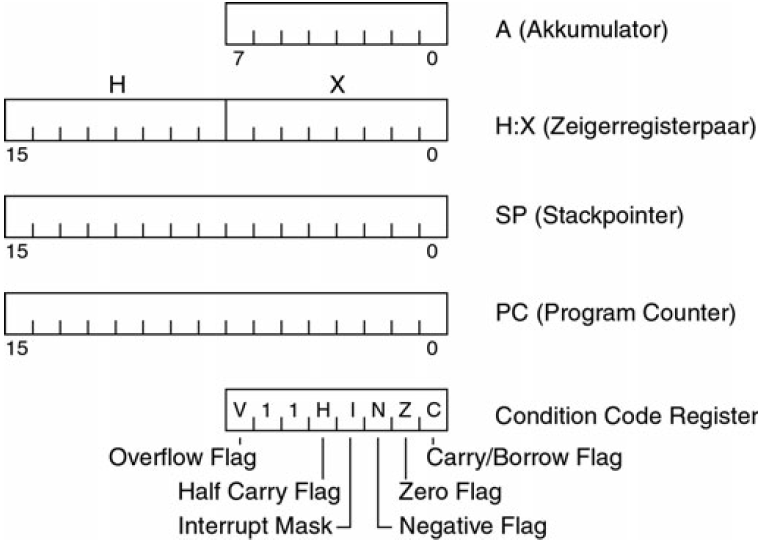
\includegraphics[width = 0.8\linewidth]{images/Plattformen/CPU08Register}
	\end{multicols}
\end{minipage}
\begin{minipage}{0.48\textwidth}
\flushleft{}
    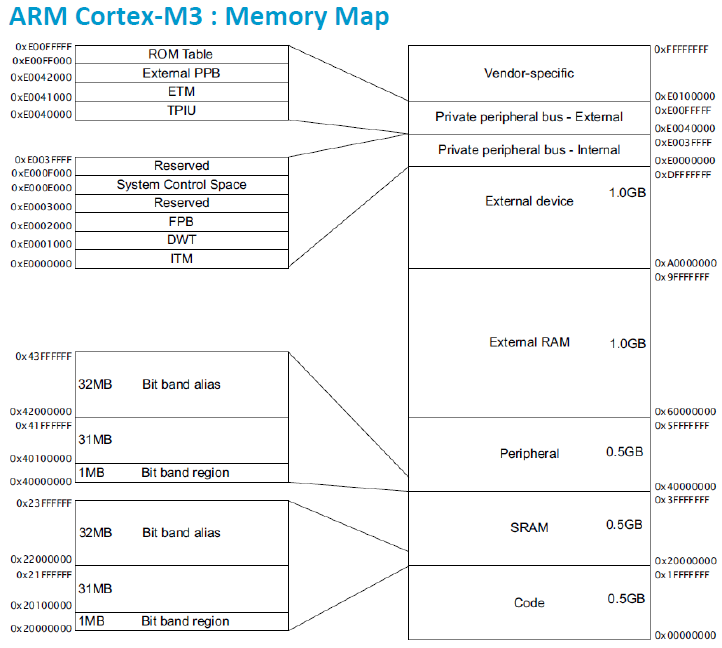
\includegraphics[width = 1\linewidth]{images/Plattformen/Cortex_M3_MMap}
\end{minipage}
\begin{minipage}{0.52\textwidth}
\flushright
    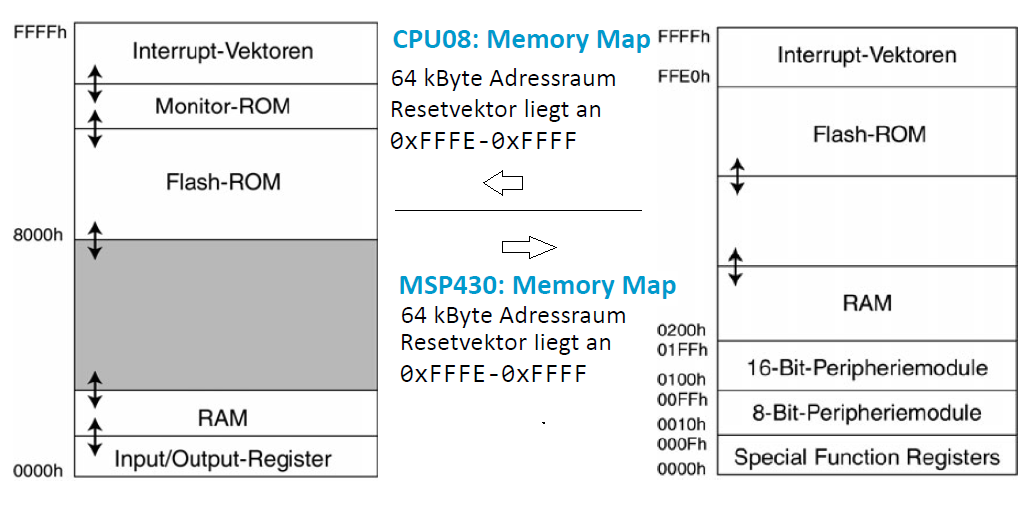
\includegraphics[width = 0.9\linewidth]{images/Plattformen/CPU08_MSP_MMap}
	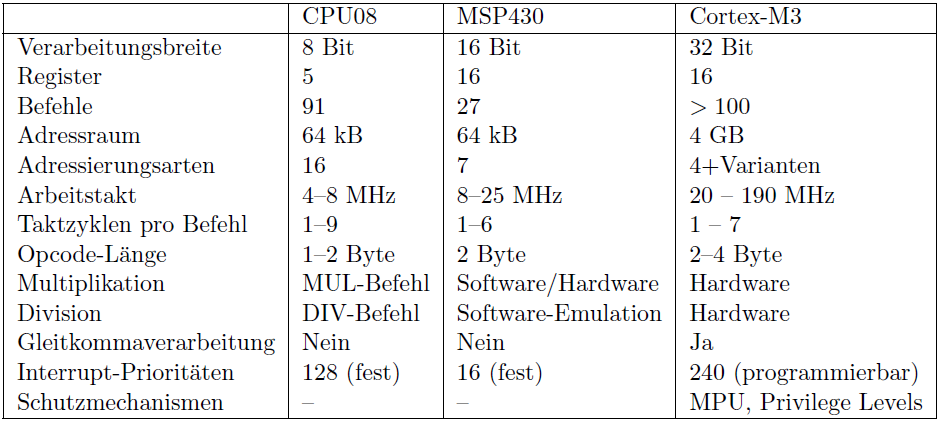
\includegraphics[width = 0.9\linewidth]{images/Plattformen/VergleichBSPArchitektur}
\end{minipage}
\subsection{Digital Signal Processor (DSP)}
\begin{multicols}{2}
\subsubsection{DSP Eigenschaften}
\begin{itemize}
    \item Mikrocontroller, der speziell für Digital Signal Processing geeignet ist
    \item Analoge Daten kontinuierlich und in Echtzeit digital verarbeiten (filtern)
    \item Für Faltung oder FFT müssen (Abtast-)Werte mit einem Gewicht multipliziert und zu einem bestehenden Wert addiert werden
    \item Diese Multiply-Add-Folge wird häufig als Multiply-Accumulate (MAC) bezeichnet
    \item Viele Daten, immer wieder dieselben Operationen
    \item Ziel eines DSPs: nicht mehr als ein Zyklus pro MAC-Operation
    \item meist Harvard: gleichzeitig Daten und Instruktionen aus dem Speicher holen
    \item Pipelining, DMA und FPU
\end{itemize}
\columnbreak
\subsubsection{TI fixed Point DSP (C28x)}
\begin{itemize}
    \item Low-cost 32-bit fixed-point processor
    \item An 8-phase protected pipeline prevents a write to and a read from the same
location from occurring out of order
    \item 32 bit Arithmetic logic unit (ALU)
    \item Address register arithmetic unit (\textbf{ARAU}) generates data- memory addresses
and increments or decrements pointers in parallel with ALU operations
    \item 32 bit multiplier performs 32 x 32 bit 2s-complement multiplication with a 64
bit result
    \item 4Gwords (1word = 16bit) data space, 4Mwords program space
\end{itemize}
\end{multicols}

\begin{minipage}{0.5\textwidth}
\subsubsection{C28x Instruction Pipeline}
\begin{itemize}
  \item Each instruction passes through eight independent phases that form an
instruction (Instr) pipeline
  \item At any given time, up to eight instructions may be active, each in a different
phase of completion
  \item pipeline-protection mechanism ensures that reads \& writes to the same location happen in the order in which they are programmed
  \item To maximize pipeline efficiency, an instruction-fetch mechanism attempts to
keep the pipeline full:
    - Its role is to fill an instruction-fetch queue \\
    - Instr-fetch mechanism: 1 32bit or 2 16bit Instr \\
    - uses 3 program-address counters:
    program counter (PC), the instruction counter (IC), and the fetch counter (FC)
\end{itemize}
\end{minipage}
\begin{minipage}{0.5\textwidth}
\end{minipage}
\begin{minipage}{0.5\textwidth}
\subsubsection{C28x Instruction Pipeline Phases}
\begin{itemize}
  \item Instruction fetch (F1 and F2) loads instr from program memory to instr-fetch queue
  \vspace{-0.8\baselineskip}
  \item Instruction decode (D1 and D2) requests an instr from the instr-fetch queue, decodes the instr, loads it into instr register, branches are taken in D2 if required (ARAU)
  \vspace{-0.8\baselineskip}
  \item Read phase (R1 and R2) reads data from memory if data has to be read
  \vspace{-0.8\baselineskip}
  \item Execute (E) CPU performs all multiplier, shifter and ALU ops
  \vspace{-0.8\baselineskip}
  \item Write (W) writes data to memory if required
\end{itemize}
 \vspace{-0.8\baselineskip}
 \subsubsection{C28x Instruction Pipeline Protection}
 \vspace{-0.8\baselineskip}
 \begin{itemize}
 \item unprotected pipeline und read\&write an selbe Stelle $\rightarrow$ Fehler (falsche Reihenfolge)
  \vspace{-0.8\baselineskip}
 \item CPU auto adds inactive cycles (NOP) to ensure that reads\&writes happen as intended
  \vspace{-0.8\baselineskip}
  \item Zwei Typen von Fehlern: 1. read\&write to same data-space location 2. Register conflicts
\end{itemize}
\end{minipage}
\begin{itemize}
 \item Branches are taken in D2: - Content in F1-D1 could then be wrong
 - This requires a flush of F1-D1 - Pipeline flushes should be avoided $\rightarrow$ machen das System langsam! (z.B. if-Abfrage in einer for-Schleife)
\end{itemize}
\subsubsection{C28x Pipeline Beispiele}
\vspace{-2\baselineskip}
\begin{minipage}{0.53\textwidth}
  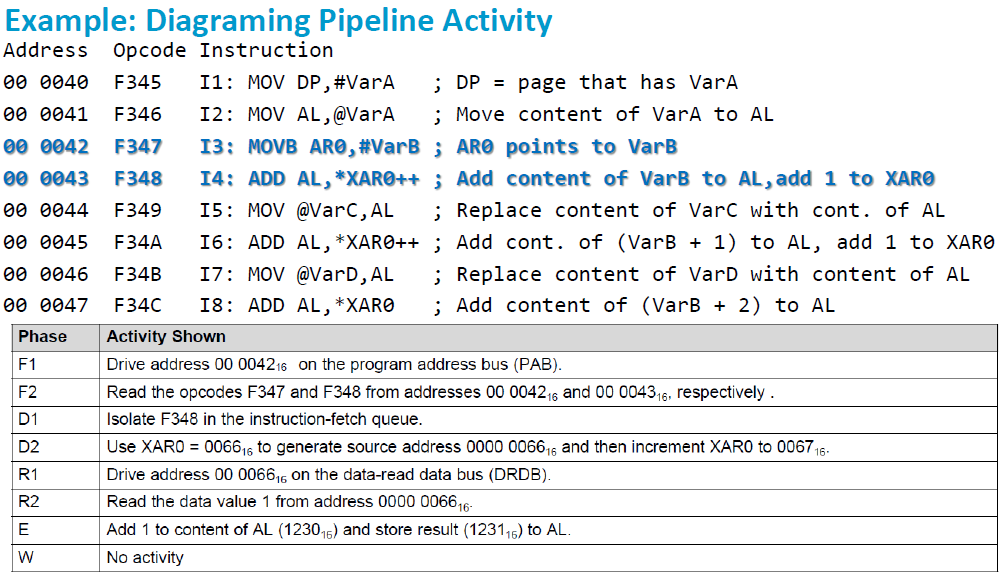
\includegraphics[width = 1\linewidth]{images/Plattformen/Example_pipeline}
\end{minipage}
\begin{minipage}{0.47\textwidth}
  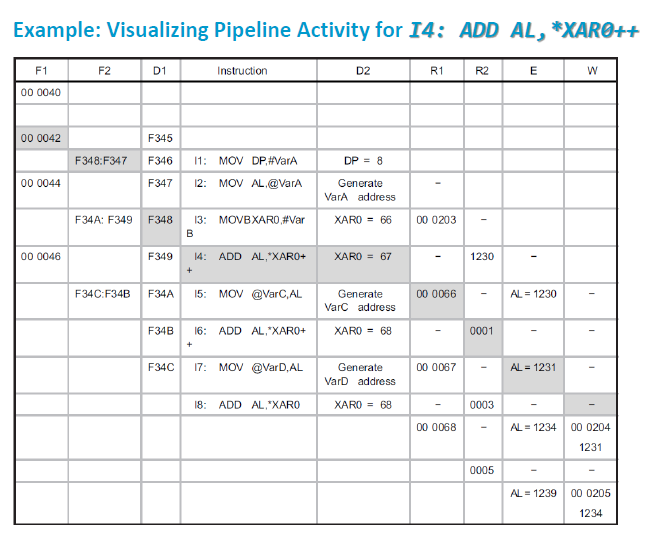
\includegraphics[width = 1\linewidth]{images/Plattformen/Example_pipeline_activity}
\end{minipage}
\begin{minipage}{0.75\textwidth}
\flushleft
  C-Code / Assembler-Code und Darstellung der Instruction Pipeline
  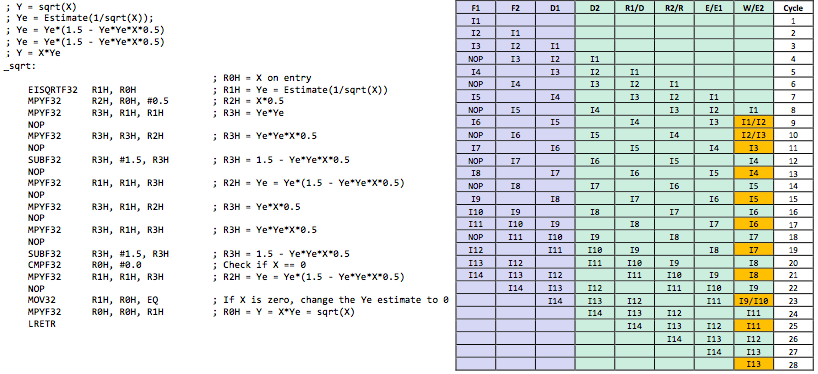
\includegraphics[width = 1\linewidth]{images/Plattformen/Example_pipeline_assembler}
\end{minipage}
\begin{minipage}{0.25\textwidth}
Gründe für Freeze in Pipeline Activity: \newline
\underline{Wait states:} Lesen von oder Schreiben ins Memory dauert länger als 1 stage \newline
Activity in the pipeline freezes depending on where the wait state occurrred (F1, R1, W)\newline
\underline{Instr not available:} if instr is not available in D2 phase.
\end{minipage}
\newpage
\begin{minipage}{0.45\textwidth}
	\subsubsection{C28x FPU Pipeline}
	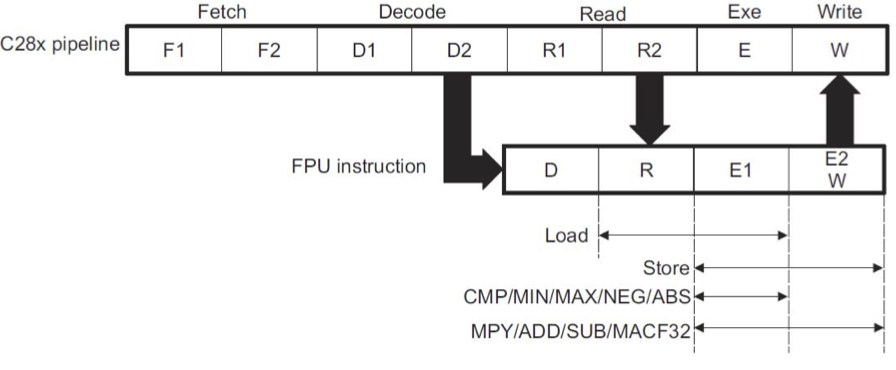
\includegraphics[width = 1\linewidth]{images/Plattformen/C28xPipeline}
\end{minipage}
\begin{minipage}{0.55\textwidth}
\subsection{ARM-Cortex}
\subsubsection{ARM-Cortex Family}
\begin{itemize}
 \item ARMv8-A: Application profile: High-performance (Smartphones, Tablets) Cortex-A72, -A57, -A53
 \item ARMv8-R: Real-time profile: Embedded applications in automotive and industrial control: Cortex-R4, -R5, -R7
 \item ARMv8-M: Microcontroller profile: Embedded applications, optimized for energy efficiency and cost Cortex-M0, -M1, -M3, -M4, -M7
\end{itemize}
\end{minipage}
\subsubsection{Cortex-M family}
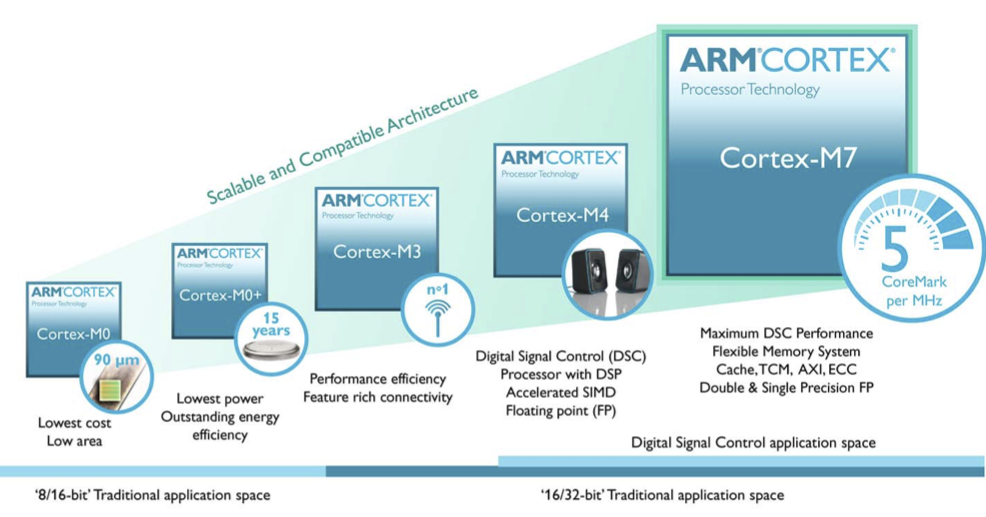
\includegraphics[width = 0.8\linewidth]{images/Plattformen/Cortex_M_Family}\newline
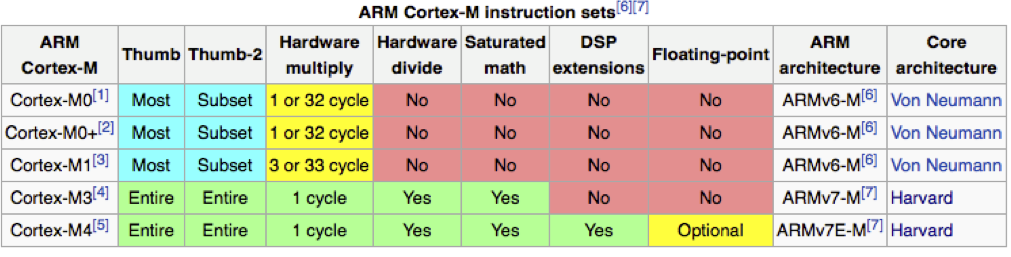
\includegraphics[width = 0.8\linewidth]{images/Plattformen/Cortex_M_instr_set}\newline
Befehle für den Cortex-M4 mit FPU (M4F) beginnen immer mit "'V"' z.B: VADD, VMUL, VDIV, VSQRT;\newline
\newline
\begin{minipage}{0.4\textwidth}
\subsection{MSP432 und Vergleich}
\begin{itemize}
  \item Successor of MSP430
  \vspace{-0.7\baselineskip}
  \item No proprietary core anymore but ARM Cortex-M4F
  \vspace{-0.7\baselineskip}
  \item Ultra-low-power (90 $\mu$A/MHz, static 25 nA)
  \vspace{-0.7\baselineskip}
  \item Wide configuration of device options is planned
\end{itemize}
\end{minipage}
\begin{minipage}{0.6\textwidth}
\includegraphics[width = 1\linewidth]{images/Plattformen/Comparison}
\end{minipage}
